\documentclass[11pt, a4paper]{article}
% \usepackage[T1]{fontenc}
\usepackage[utf8]{inputenc}
\usepackage{listings}
\usepackage[margin=1.0in]{geometry}
\usepackage{color}
\usepackage{graphicx}
\usepackage{tabularx}
\usepackage{url} 

\title{DMS Dokumenten Management System}
\author{Melanie Göbel, Gary Ye (4BHIT)}
\date{\today{}, Wien}

\begin{document}

\lstset{ %
  backgroundcolor=\color{white},   % choose the background color; you must add \usepackage{color} or \usepackage{xcolor}
  basicstyle=\footnotesize,        % the size of the fonts that are used for the code
  breakatwhitespace=false,         % sets if automatic breaks should only happen at whitespace
  breaklines=true,                 % sets automatic line breaking
  captionpos=b,                    % sets the caption-position to bottom
% commentstyle=\color{mygreen},    % comment style
  deletekeywords={...},            % if you want to delete keywords from the given language
  escapeinside={\%*}{*)},          % if you want to add LaTeX within your code
  extendedchars=true,              % lets you use non-ASCII characters; for 8-bits encodings only, does not work with UTF-8
% frame=single,                    % adds a frame around the code
  keepspaces=true,                 % keeps spaces in text, useful for keeping indentation of code (possibly needs columns=flexible)
% keywordstyle=\color{blue},       % keyword style
% language=bash,                   % the language of the code
  morekeywords={*,...},            % if you want to add more keywords to the set
  numbersep=5pt,                   % how far the line-numbers are from the code
  rulecolor=\color{black},         % if not set, the frame-color may be changed on line-breaks within not-black text (e.g. comments (green here))
  showspaces=false,                % show spaces everywhere adding particular underscores; it overrides 'showstringspaces'
  showstringspaces=false,          % underline spaces within strings only
  showtabs=false,                  % show tabs within strings adding particular underscores
  tabsize=2,                       % sets default tabsize to 2 spaces
  title=\lstname                   % show the filename of files included with \lstinputlisting; also try caption instead of title
}


\maketitle
\newpage
\tableofcontents
\newpage

\section{Aufgabenstellung}

\subsection*{Dokumenten Management System}

Ein Dokumenten Management System (kurz DMS genannt) erlaubt das zentrale Speichern von beliebigen Dokumenten. Dokumente können somit gezielt an einem Platz gesucht und administriert werden. Eine zentrale Aufgabe eines DMS ist es den Verlauf eines Dokuments aufzuzeichnen und jederzeit abrufen zu können.

\subsection*{Suche / Indizierung}

Ein DMS ist nur so gut, wie seine Suchfunktion. Es soll daher möglich sein nach folgenden Parametern zu suchen.

\begin{itemize}
\item Autor
\item Kategorie
\item Kommentar
\item Dokumentname
\item Dokumenttyp
\item Schlüsselwörter
\end{itemize}
Diese Parameter beschreiben auch die Eigenschaften eines Dokuments in dem DMS.

\subsection*{Authentifikation / Autorisierung}

Bei dem DMS soll es sich um ein rollenbasiertes System handeln. Folgende Rollen sollen im System implementiert werden:

\subsubsection*{Administrator}
Der Administrator hat alle Rechte und kann auf alle Dokumente zugreifen.

\subsubsection*{Dokumentbesitzer}
Jener Benutzer der ein Dokument im DMS erstmalig erfasst, wird als Dokument Besitzer vermerkt.

\subsubsection*{Dokumentnutzer}
Der Administrator und der Dokumentbesitzer kann beliebigen andere Benutzer den Zugriff auf das Dokument gewähren.
Zur Vereinfachung wird beim Zugriff nicht zwischen Lese- und Schreibrechten unterschieden, sprich Zugriff auf ein Dokument bedeutet Lese- und Schreibzugriff.

\subsection*{Verlauf}

Für jedes Dokument in dem DMS soll mit einer Versionsnummer versehen und gespeichert werden. Jede Änderung des Dokuments führt dazu, dass die Versionsnummer um eins erhöht wird. Alle Änderungen werden mit folgenden Parameter im DMS gespeichert:

\begin{itemize}
\item Versionsnummer
\item Benutzer
\item Datum / Uhrzeit
\item Kommentar
\end{itemize}

\subsection*{Upload / Download}

Das DMS soll in dieser Version folgende Aktionen erlauben:

\subsubsection*{Upload}
Ein neues bzw. eine neue Version eines Dokuments werden im DMS abgelegt und die Versionsnummer wird um eins erhöht. Ebenso wird der Verlauf um diese Aktion erweitert. Wenn das Dokument zuvor von dem Benutzer heruntergeladen wurde, so führt der Upload zu einer Freigabe des Dokuments, wodurch anderen Dokumentennutzer das Dokument bearbeiten können. Es kann immer nur ein Dokument hochgeladen werden. Ein Hochladen mehrerer Dokumente bzw. ganzer Verzeichnisstrukturen sind in der nächsten Ausbaustufe angedacht.

\subsubsection*{Checkout / Download}
Ein Checkout eines Dokuments führt gleichzeitig dazu, dass das Dokument im DMS als GESPERRT vermerkt wird. Diese Sperre gilt für alle anderen Benutzer und kann nur von dem Dokumentnutzer durch einen UPLOAD einer neuen Version bzw. mit Hilfe der GUI durch den Dokumentbesitzer bzw. Administrator freigegeben werden.

\subsubsection*{Löschen}
Ein bestehendes Dokument kann nur gelöscht werden, wenn es nicht gesperrt ist. Das Löschen des Dokuments erfolgt auch physisch und führt dazu das alle Einträge im DMS (Bsp. Verlauf, Dokumentbenutzer, etc.) gelöscht werden.



Erstelle mit Hilfe der Frameworks JEE oder Play eine Webapplikation, die die Funktionalität dieses Dokumentenmanagementsystems abbildet. Verwende das ORM Framework Hibernate um die Daten des Dokuments in einer Datebank abzuspeichern. Führe zu Beginn der Arbeit eine ausführliche Analyse \& Designphase durch, um die Problem noch vor der Implementierung mit den Projektmitgliedern abzuklären.

\section{Designüberlegung}

Aus Flexibilitäts Gründen wurde der Dokument-Typ und die Dokument-Kategorie ausgelegt und als Enum realisiert. Wenn auf ein Dokument zugegriffen wird,
soll dieses gelockt sein, dies realisieren wir mit einer boolean Variable in der Document Klasse. Um das Document zu verwalten besteht eine Komposition zwischen Document und DocumentVersion. Ein Document hat nämlich mehrere Versionen. Eine Version steht immer im Zusammenhang zu einem User, da es immer einen Editor gab.

Zur Authentifikation und Autorisierung haben wir vor Apache Shiro zu verwenden. Apache Shiro ist ein Java Sicherheits Framework, das Authentifikation, Autorisierung,
Kryptographie, uvm. unterstützt.

\subsection{Domänenmodell}
Das Analyse und das Design wurde mittels eines UML Klassen Diagrams realisiert.

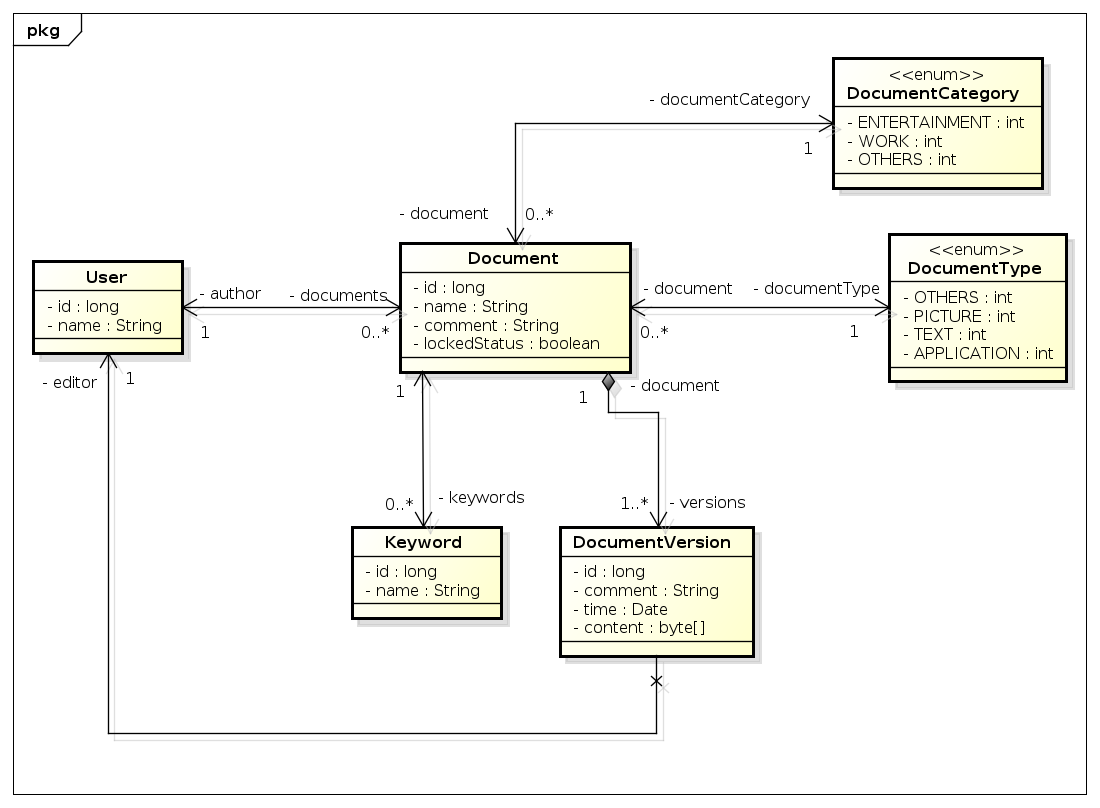
\includegraphics[width=\textwidth]{pic/dms-begin}

Am Ende schaut das Model folgendermaßen aus:

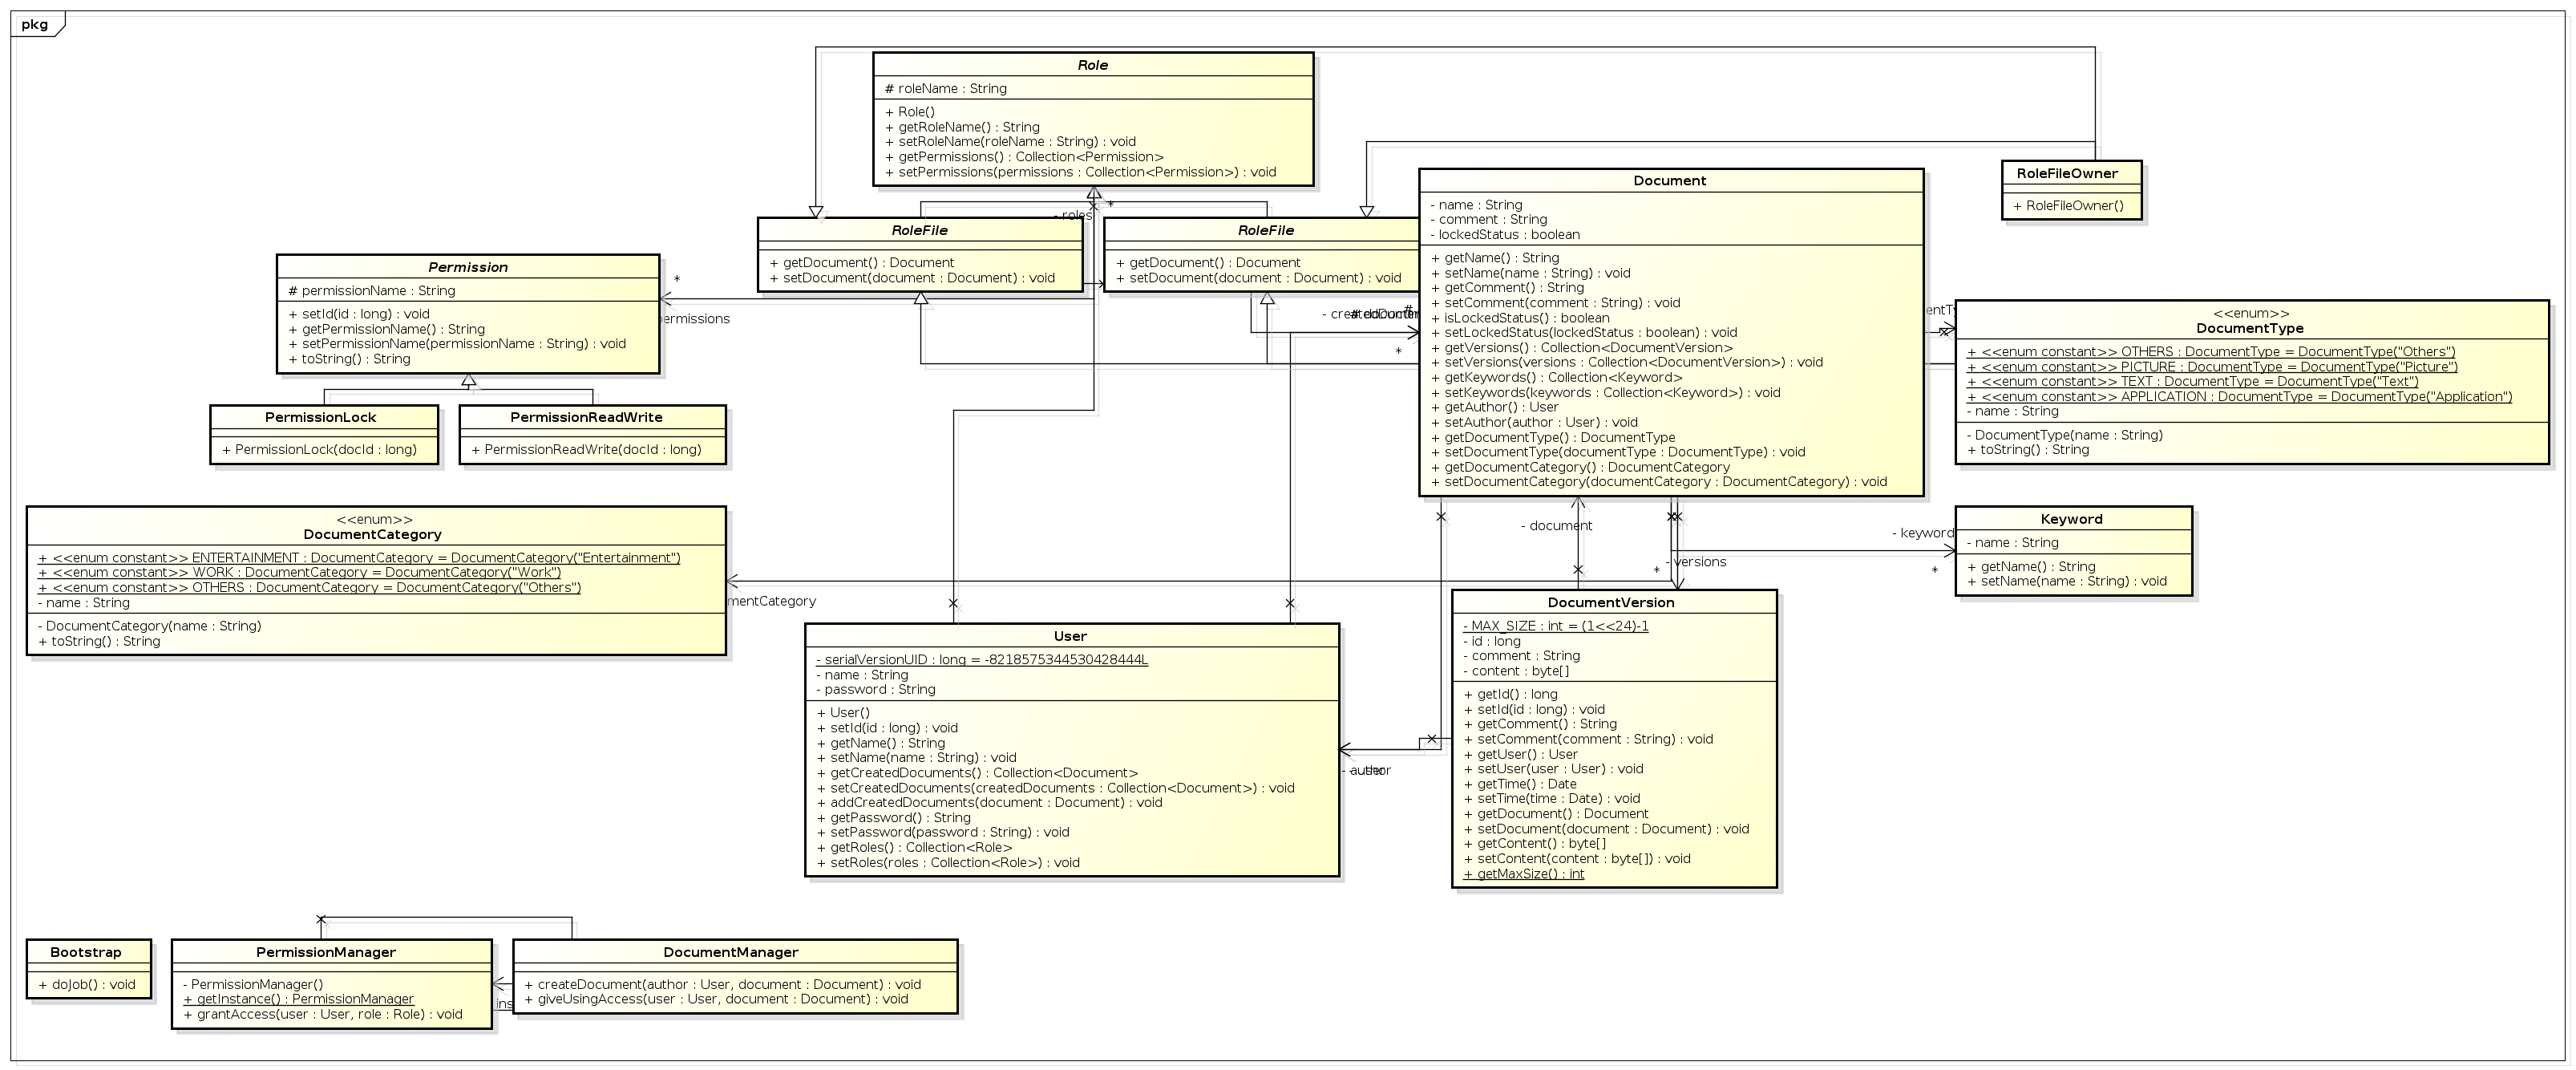
\includegraphics[width=\textwidth]{pic/dms-end}

Die Klassen bezüglich RBAC wurden bei der Planung nicht beachtet, da diese Technologie sehr neu war. Außerdem wurde vor der Planung für das Shiro Framework entschieden und davor ist der Aufbau der benötigten Klassen nicht bekannt gewesen.

\subsection{Technologien}

Es wurde beschlossen das Play Web Framework zu verwenden. Desweiteren wurde, da es auch verlangt wurde, das ORM Framework Hibernate eingesetzt. Für die Authentifikation und Autorisierung wurde für das Shiro Framework entschieden, da es nicht zu komplex wirkt und gut für die Applikation ausmacht. 

Als Datenbank wurde die MySQL Datenbank ausgewählt, da sehr viel Erfahrung damit besteht.
% TODO: Shiro http://shiro.apache.org/java-authentication-guide.html
% TODO: Hibernate http://hibernate.org/ 
% TODO: Play http://playframework.com

\section{Arbeitsaufteilung}

Es wurde beschlossen alle Features zu implementieren, daher sind die Arbeitsaufteilung wie gefolgt. 

\begin{itemize}
  \item Domänenmodell werden von beiden Teammitgliedern designed.
  \item Authentifikation und Autorisierung wird von Gary Ye durchgeführt.
  \item GUI Oberfläche wird von Melanie Göbel gestaltet.
  \item Unit Testing wird von Gary Ye durchgeführt.
  \item Functional Testing wird von Melanie durchgeführt.
\end{itemize}

\section{Aufwandsschätzung}

\subsection*{Melanie Göbel}
\begin{center}
  \begin{tabular}{| l | l | l |}
    \hline
    Task & Geschätzt & Tatsächlich \\ \hline    
		Grafische Oberfläche & 5 & 2 \\ \hline
		Gesamt & 5 & 2 \\ \hline
  \end{tabular}
\end{center}


\subsection*{Gary Ye}
\begin{center}
  \begin{tabular}{| l | l | l |}
    \hline
    Task & Geschätzt & Tatsächlich \\ \hline
    Domänenmodell Design & 2h & 1.5h \\ \hline
		Domänenmodell Implementierung & 1h & 4h \\ \hline
    Authentifikation und Autorisierung & 3h & 6h \\ \hline
		Gesamt & 6 & 11.5 \\ \hline
  \end{tabular}
\end{center}

\section{Vorbereitung und Installation}
\subsection{Play}

Mit Play einfach eine neue Applikation erstellen. (Es wird angenommen, dass Play schon wegen der vorigen Übung erfolgreich auf dem System installiert ist)

\begin{lstlisting}
> play new dms
\end{lstlisting}

Integration mit Eclipse erfolgt mit 

\begin{lstlisting}
> play eclipse
\end{lstlisting}

In Play 1.2.7 erfolgt es mit

\begin{lstlisting}
> play eclipsify
\end{lstlisting}

\subsection{Play Konfiguration mit MySQL}

Damit Play im Hintergrund mit MySQL arbeitet, müssen einige Änderungen vorgenommen werden.

\subsubsection*{Datenbank erstellen}

Folgende Befehle müssen zuerst in der Datenbank durchgeführt werden.

\begin{lstlisting}
mysql>CREATE DATABASE dms;
mysql>GRANT ALL PRIVILEGES ON dms.* TO 'dmsuser'@'%' IDENTIFIED BY 'dmspassword';
mysql>FLUSH PRIVILEGES;\end{lstlisting}

\subsubsection*{application.conf (Play 2.x)}

In dem File müssen wir die JDBC Einstellungen an die zu verwendende Datenbank anpassen. Hierbei verbinden wir uns mit der MySQL Datenbank namens "dms", die auf dem Server mit dem Hostnamen "ubuntu-vm" liegt. 

\begin{lstlisting}
db.default.driver=com.mysql.jdbc.Driver
db.default.url="jdbc:mysql://ubuntu-vm/dms"
db.default.user=dmsuser
db.default.password=dmspassword\end{lstlisting}

\subsubsection*{build.sbt}

Auch hier muss eine Zeile hinzugefügt werden, damit der MySQL Treiber auch verwendet wird.
\begin{lstlisting}
libraryDependencies ++= Seq(
  ...
	"mysql" % "mysql-connector-java" % "5.1.18",
}\end{lstlisting}

\subsection{JPA (Hibernate) (Play 2.x)}

\subsubsection*{build.sbt}

\begin{lstlisting}
libraryDependencies ++= Seq(
  ...
	javaJpa,
	"org.hibernate" % "hibernate-entitymanager" % "4.2.2.Final"
}\end{lstlisting}

\subsubsection*{application.conf}

Die folgenden Zeilen müssen hinzugefügt werden.

\begin{lstlisting}
jpa.default=defaultPersistenceUnit
db.default.jndiName=DefaultDS
\end{lstlisting}

\subsubsection*{persistence.xml}

Das File sollte im conf/META-INF Ordner liegen.

\begin{lstlisting}
<?xml version="1.0"?>
<persistence xmlns="http://java.sun.com/xml/ns/persistence" xmlns:xsi="http://www.w3.org/2001/XMLSchema-instance" xsi:schemaLocation="http://java.sun.com/xml/ns/persistence http://java.sun.com/xml/ns/persistence/persistence_2_0.xsd" version="2.0">
  <persistence-unit name="defaultPersistenceUnit" transaction-type="RESOURCE_LOCAL">
    <!-- <provider>org.hibernate.ejb.HibernatePersistence</provider>
    <non-jta-data-source>DefaultDS</non-jta-data-source> -->
    <properties>
      <property name="hibernate.connection.driver_class" value="com.mysql.jdbc.Driver"/>
      <property name="hibernate.connection.url" value="jdbc:mysql://ubuntu-vm:3306/dms"/>
      <property name="hibernate.connection.username" value="dmsuser"/>
      <property name="hibernate.connection.password" value="dmspassword"/>
      <property name="hibernate.dialect" value="org.hibernate.dialect.MySQL5InnoDBDialect"/>
      <property name="hibernate.show_sql" value="false"/>
      <property name="hibernate.hbm2ddl.auto" value="create"/>
    </properties>
  </persistence-unit>
</persistence>
\end{lstlisting}

\section{Neue Technologie}

\subsection{Apache Shiro}

Apache Shiro ist ein Framework für Authentifizierung und Autorisierung. Außerdem beinhaltet es Features wie Caching, Session und Kryptografie. 

\section{Testbericht}
\subsection{Testing in Play 1.2.7}

Getestet wurde mit Hilfe einer JUnit Erweiterung von Play, die einem "Fixture" anbietet. Man kann jede vor jedem Testcase die Datenbank auf einen bestimmten Zustand setzen, damit ein Testcase nicht von vorherigen Testcases beeinträchtigt wird.

Im Test Verzeichnis wurden mehrere yml Files angelegt, diese sind yml Files, die die Datenbank beschreiben. Die Syntax ist sehr einfach und findet man unter. % TODO cite yml  

Als Beispiel wurde hier das yml für das Testen der Authentifizierung verwendet.

\begin{lstlisting}
User(gary):
  name: "gary"
  password: "password"

User(tom):
  name: "tom"
  password: "letmein"
\end{lstlisting}

Hier wurden zwei Users erstellt, wobei der erste den Variablennamen (den man in den Klammern neben der Klassenname stehen hat) "gary" hat. 

Dabei muss man auf einige Bedinungen achten:
\begin{itemize}
	\item Es dürfen keine Tabs für Einrückungen verwendet werden, stattdessen benutzt man die alte Variante, nämlich die Leerzeichen.
	\item Die Model klassen müssen im Package models liegen. Es gab am Anfang ein Problem, weil das Package "model" hieß und die Klassen konnten nicht gefunden werden.
\end{itemize}

Mit der grafischen Oberfläche kann man ganz leicht auswählen, welche Tests zu testen sind.

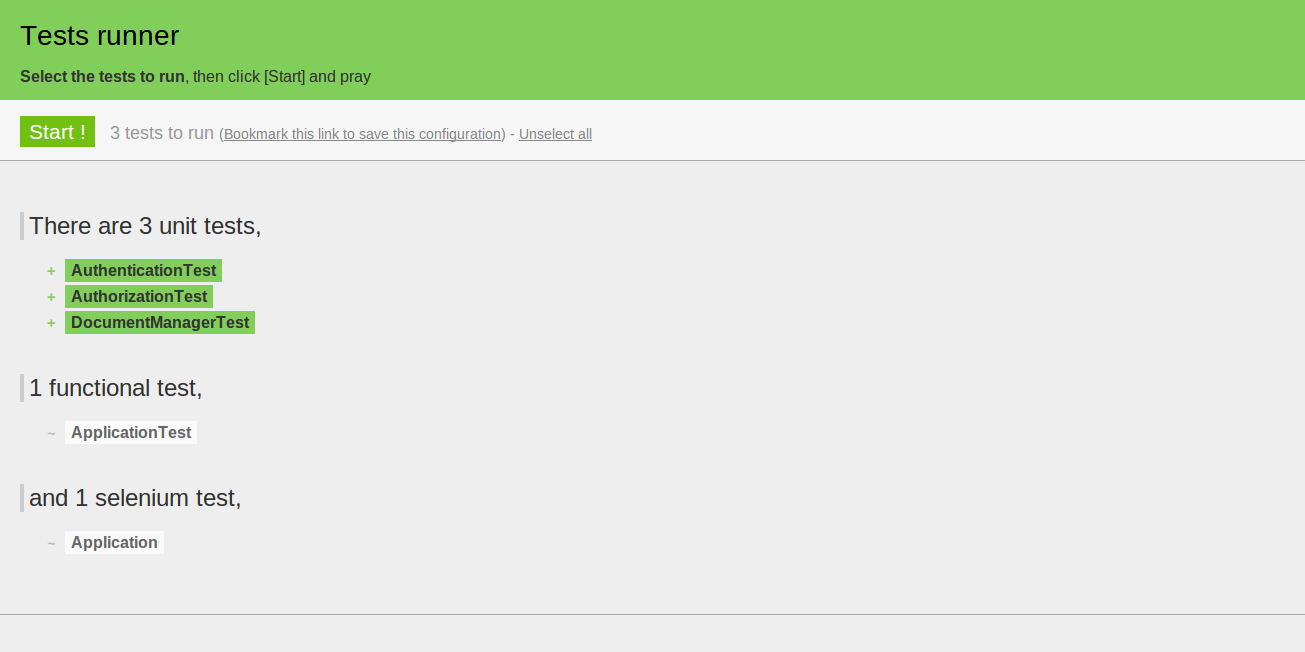
\includegraphics[width=\textwidth]{pic/play-test}

\section{Aufgetretene Probleme}
\subsection{Play Version inkompatibel mit JPA}
Ab Play 2.x wurden viele Klassen wie z.B. jpa.db.jpa.Model entfernt, daher mussten wir zu Play 1.2.7 Version wechseln, da sie diese Klasse und vieles mehr unterstützt. Dies hat sehr viel Zeit gekostet, da die Konfiguration in den beiden Versionen nicht gleich waren. 
\subsection{Play Testing Bug}
Nachdem man "play test" zum Testen ausgeführt hat, so sollte man keinen Code verändern, da die Applikation neu gestartet wird. Danach funktioniert die Authentifizierung nicht mehr.
\subsection{One To Many add}
Wenn man bei einer 1:N Beziehung nur auf einer Seite das Objekt der anderen Seite setzt, so wird das nicht automatisch auf der anderen Seite durchgeführt. Das Konkrete Problem war, der User hat ein Dokument zu seinen erstellten Dokumenten hinzugefügt. Jedoch steht dann im hinzugefügten Dokument nicht, wer der Autor war.

Die Lösung dazu ist, dass man das Setzen auf beiden Seiten wie in % TODO: http://en.wikibooks.org/wiki/Java_Persistence/Relationships#Object_corruption.2C_one_side_of_the_relationship_is_not_updated_after_updating_the_other_side
beschrieben durchführt.

Bei N:M Beziehung tritt dieser Fall nicht auf.

\section{Resultate und Niederlagen}
% \bibliography{protokoll}{}
% \bibliographystyle{plain}
\end{document}
